\documentclass[12pt, a4paper]{article}

\usepackage[a4paper, top=2.5cm, bottom=2.5cm, left=2.5cm, right=2.5cm]{geometry}
\usepackage{graphicx}
\usepackage{amsmath}
\usepackage{amssymb}
\usepackage{float}
\usepackage{booktabs}
\usepackage{parskip}
\usepackage{siunitx}
\usepackage{enumitem}
\usepackage[hidelinks]{hyperref}
\usepackage{titlesec}
\usepackage{fancyhdr}

\pagestyle{fancy}
\fancyhf{}
\rhead{42059/41034 --- Lab 5}
\lhead{D-Latch Simulation}
\cfoot{\thepage}

\titleformat{\section}{\large\bfseries}{}{0em}{}[\titlerule]
\titleformat{\subsection}{\normalsize\bfseries}{}{0em}{}

\graphicspath{{./}}
\usepackage{grffile}

\begin{document}

\begin{titlepage}
    \centering
    \vspace*{2cm}
    {\LARGE\bfseries 42059 / 41034 --- Lab 5 Report\par}
    \vspace{0.5cm}
    {\Large D-Latch Simulation with T-Spice\par}
    \vspace{1.5cm}
    \begin{tabular}{rl}
        \textbf{Student Name:} & Nathan Nguyen       \\[0.4em]
        \textbf{Student ID:}   & 24493999         \\[0.4em]
        \textbf{Session:}      & Autumn 2026  \\[0.4em]
        \textbf{Date:}         & 20 March 2026 \\
    \end{tabular}
    \vfill
    {\small University of Technology Sydney}
\end{titlepage}

%------------------------
\section{Exercise 1: D-Latch Circuit Design and Simulation}
%------------------------

A D (Data or Transparent) latch is a 1-bit memory element with a data input D, a clock signal CLK, and complementary outputs Q and $\bar{Q}$. When CLK is HIGH the latch is transparent and Q follows D; when CLK is LOW the latch holds its last state regardless of changes on D. The characteristic table is shown in Table~\ref{tab:dlatch_truth}.

\begin{table}[H]
    \centering
    \caption{D-latch characteristic table.}
    \label{tab:dlatch_truth}
    \begin{tabular}{ccc}
        \toprule
        CLK & D & $Q(t+1)$ \\
        \midrule
        0 & x & $Q(t)$ \\
        1 & 0 & 0 \\
        1 & 1 & 1 \\
        \bottomrule
    \end{tabular}
\end{table}

The D-latch was implemented in S-Edit using four NAND gates and one inverter from Lab~3. The inverter produces $\overline{\text{CLK}}$, which drives the reset NAND path, while the data path uses the non-inverted CLK. The resulting schematic is shown in Figure~\ref{fig:dlatch_schem}.

\textbf{[FLAG: D-latch schematic screenshot not provided --- place dlatch\_schem.png in the same folder as this report.]}

\begin{figure}[H]
    \centering
    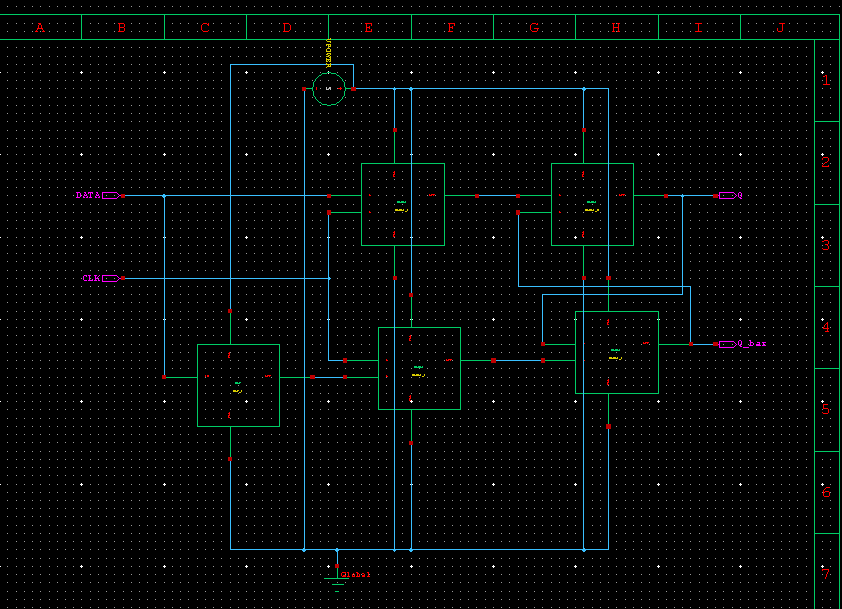
\includegraphics[width=\textwidth]{dlatch_schem.png}
    \caption{D-latch schematic in S-Edit using four NAND gates and one inverter.}
    \label{fig:dlatch_schem}
\end{figure}

The circuit was simulated with a DATA pulse of period 20\,ns and a CLK pulse of period 40\,ns ($V_{DD} = 5$\,V). The resulting waveforms are shown in Figure~\ref{fig:dlatch_transient}.

\textbf{[FLAG: D-latch transient waveform not provided --- place dlatch\_transient.png in the same folder as this report.]}

\begin{figure}[H]
    \centering
    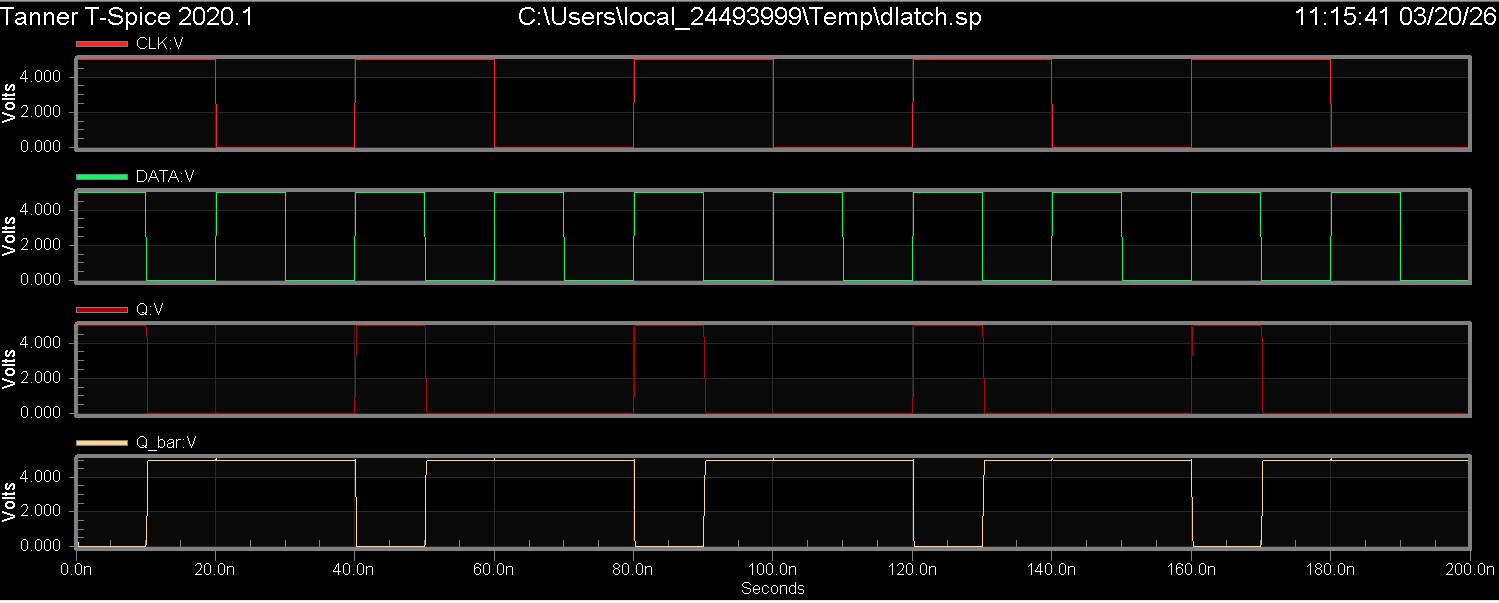
\includegraphics[width=\textwidth]{dlatch_transient.png}
    \caption{T-SPICE transient simulation of the D-latch. When CLK is HIGH, Q follows DATA; when CLK is LOW, Q retains its last value.}
    \label{fig:dlatch_transient}
\end{figure}

The waveforms confirm correct D-latch behaviour: Q tracks DATA only during HIGH CLK phases, and $\bar{Q}$ is always the complement of Q.

%------------------------
\section{Exercise 2: Propagation Delay}
%------------------------

The propagation delay from DATA to Q was measured with CLK held HIGH (DC 5\,V) so that the latch remains transparent. The \texttt{.MEASURE} command captured the rising delay ($t_{pd\_r}$) and falling delay ($t_{pd\_f}$), both measured at the 50\% ($V_{DD}/2 = 2.5$\,V) threshold on the third switching cycle to avoid start-up transients.

\textbf{[FLAG: tpd\_r and tpd\_f measurement results not provided --- please insert T-SPICE .MEASURE output here.]}

\begin{table}[H]
    \centering
    \caption{D-latch propagation delay from DATA to Q.}
    \label{tab:dlatch_delay}
    \begin{tabular}{ccc}
        \toprule
        $t_{pd\_r}$ (ps) & $t_{pd\_f}$ (ps) & $t_{pd(avg)}$ (ps) \\
        \midrule
        [FLAG] & [FLAG] & [FLAG] \\
        \bottomrule
    \end{tabular}
\end{table}

The average propagation delay is:
\[
    t_{pd(avg)} = \frac{t_{pd\_r} + t_{pd\_f}}{2}
\]

$t_{pd\_f} > t_{pd\_r}$ because the falling transition at Q must discharge through the series NMOS stack in the NAND gate, which presents higher resistance than the parallel PMOS pull-up network driving the rising transition.

%------------------------
\section{Exercise 3: Average Power Consumption}
%------------------------

Average power consumption was measured with the clock restored to a pulse source (period 40\,ns). The \texttt{.MEASURE} command computed the average supply current $I_{avg}$ from \texttt{VVPOWER} and the average power $P_{avg} = -5 \times I_{avg}$ (the negative sign corrects for the SPICE convention where current flowing into the supply is reported as negative).

\textbf{[FLAG: Iavg and Pavg measurement results not provided --- please insert T-SPICE .MEASURE output here.]}

\begin{table}[H]
    \centering
    \caption{D-latch average power consumption at 25\,MHz clock (period 40\,ns).}
    \label{tab:dlatch_power}
    \begin{tabular}{cc}
        \toprule
        $I_{avg}$ ($\mu$A) & $P_{avg}$ ($\mu$W) \\
        \midrule
        [FLAG] & [FLAG] \\
        \bottomrule
    \end{tabular}
\end{table}

%------------------------
\section{Exercise 4: Power vs.\ Clock Frequency}
%------------------------

To verify that dynamic power consumption scales linearly with frequency ($P \propto f$), the simulation was repeated at different clock frequencies by varying the period parameter of the CLK pulse source. The results are summarised in Table~\ref{tab:dlatch_power_freq}.

\textbf{[FLAG: Power vs.\ frequency measurement results not provided --- please insert T-SPICE .MEASURE output for each clock period here.]}

\begin{table}[H]
    \centering
    \caption{Average power consumption vs.\ clock frequency.}
    \label{tab:dlatch_power_freq}
    \begin{tabular}{cccc}
        \toprule
        Period (ns) & Frequency (MHz) & $I_{avg}$ ($\mu$A) & $P_{avg}$ ($\mu$W) \\
        \midrule
        20  & 50   & [FLAG] & [FLAG] \\
        40  & 25   & [FLAG] & [FLAG] \\
        80  & 12.5 & [FLAG] & [FLAG] \\
        160 & 6.25 & [FLAG] & [FLAG] \\
        \bottomrule
    \end{tabular}
\end{table}

As clock frequency increases, more charge/discharge cycles occur per second, causing $P_{avg}$ to increase proportionally. This is consistent with the dynamic power model $P_{dyn} = \alpha C_L V_{DD}^2 f$, where $\alpha$ is the activity factor.

\end{document}
